% ---
% filename : ["electrotechnique_electromagnetisme_20260428_421_electroaimant_u.tex"]
% id : "electrotechnique_electromagnetisme_20260428_421"
% title : "Électroaimant en U et polarité"
% domain : "Électrotechnique"
% subdomain : "Électromagnétisme"
% tags : ["électroaimant", "champ magnétique", "ferromagnétisme", "bobine", "polarité", "ts"]
% difficulty : 2
% time_solve : 20
% has_octave : True
% octave_files : ["electrotechnique_electromagnetisme_20260428_421_electroaimant_u.m"]
% author : "om"
% ---
\documentclass[a4paper,11pt,answers,addpoints]{exam}

% ---------------------------------------------------------
% LANGUE, ENCODAGE, FONTS
% ---------------------------------------------------------
\usepackage[utf8]{inputenc}

% ---------------------------------------------------------
% GÉOMÉTRIE ET MISE EN PAGE
% ---------------------------------------------------------
\usepackage[left=1.7cm,right=1.5cm,top=2cm,bottom=1cm]{geometry}
%\usepackage{a4wide}
\usepackage{microtype}      % Meilleure répartition du texte
\usepackage{float}          % Positionnement [H]
\usepackage{needspace}      % Saut conditionnel intelligent

% Éviter les veuves/orphelines (optionnel, à décommenter si besoin)
% \widowpenalty=10000
% \clubpenalty=10000

% Espacement vertical flexible
%\raggedbottom
%\setlength{\parskip}{0.5em plus 0.2em minus 0.1em}
%\setlength{\parindent}{0pt}


% ---------------------------------------------------------
% MATHÉMATIQUES
% ---------------------------------------------------------
\usepackage{amsmath, amssymb, bm, esvect}

% Vecteurs
\newcommand{\V}{\overrightarrow}
\def\vect#1{\overrightarrow{\strut#1}}
\providecommand{\Degrees}[0]{\ensuremath{^\circ}}

% ---------------------------------------------------------
% UNITÉS ET GRANDEURS (SIunitx)
% ---------------------------------------------------------
\usepackage{siunitx}
\sisetup{output-decimal-marker={,}}
\DeclareSIUnit \var {var}
\DeclareSIUnit \VA {VA}
\DeclareSIUnit \kVA {kVA}
\DeclareSIUnit[quantity-product={}] \degree{\text{\textdegree}}

% ---------------------------------------------------------
% GRAPHIQUES : TikZ + CircuitikZ + PGFPlots
% ---------------------------------------------------------
\usepackage{tikz}
\usetikzlibrary{
	arrows.meta,
	intersections,
	decorations.pathreplacing,
	calligraphy,
	positioning
}

\usepackage[european,straightvoltages,EFvoltages]{circuitikz}

\usepackage{tkz-fct}
\usepackage{pgfplots}
\pgfplotsset{compat=1.12}

% Symbole étoile-triangle personnalisé
\newcommand{\wye}{%
	\mathbin{\tikz[x=1ex,y=1ex]{%
			\draw[line width=.1ex] (0,0)--(45:1)--++(-45:1) (45:1)--++(0,1);
	}}%
}


\usepackage{sankey}

\pgfdeclarelayer{background}
\pgfdeclarelayer{foreground}
\pgfdeclarelayer{sankeydebug}
\pgfsetlayers{background,main,foreground,sankeydebug}


% ---------------------------------------------------------
% TABLEAUX
% ---------------------------------------------------------
\usepackage{tabularx}
\usepackage{tabu}

% ---------------------------------------------------------
% HYPERLIENS
% ---------------------------------------------------------
\usepackage[colorlinks=true,
menucolor=red,
breaklinks=true,
urlcolor=blue,
linkcolor=blue]{hyperref}

% ---------------------------------------------------------
% COMMANDES PERSONNELLES
% ---------------------------------------------------------
\newcommand\nomauteur{bdminasmorgul@protonmail.com}
\newcommand\dateTe{28.04.2026}
\newcommand\brancheTe{TS}

% ---------------------------------------------------------
% STYLE DE L'EXERCICE
% ---------------------------------------------------------
\pagestyle{headandfoot}
\firstpageheadrule
\runningheadrule

\firstpageheader{\brancheTe\ (\nomauteur)}{Élève : }{(\dateTe) \thepage/\numpages}
\runningheader{\brancheTe\ (\nomauteur)}{Élève : }{(\dateTe) \thepage/\numpages}

% Compteur en bas de page
\newcommand{\totalpointtts}{%
	\begin{tikzpicture}[remember picture, overlay]
		\node[anchor=south west, inner sep=0pt, outer sep=0pt]
		at ([xshift=0.5cm,yshift=0.5cm]current page.south west)
		{\rotatebox{90}{Total des points : \numpoints}};
	\end{tikzpicture}
}

\firstpagefooter{\totalpointtts}{}{}
\runningfooter{\totalpointtts}{}{}

% Réglages exam
\printanswers
\addpoints
\pointsinmargin
\bracketedpoints

% ---------------------------------------------------------
% LISTINGS (code)
% ---------------------------------------------------------
\usepackage{xcolor}
\usepackage{listings}

\lstdefinestyle{octavestyle}{
	language=Matlab,
	basicstyle=\ttfamily\small,
	keywordstyle=\color{blue},
	commentstyle=\color{green!50!black},
	stringstyle=\color{red},
	stepnumber=1,
	frame=single,
	breaklines=true,
	breakatwhitespace=true,
	tabsize=4
}
\usepackage{enumitem}
% Réglage global : toutes les listes enumerate (niveau 1) en a), b), c), ...
\setlist[enumerate,1]{label=\alph*), ref=\alph*)}
\newenvironment{explication}{%
	\par\noindent\textbf{Explication. }\itshape
}{\par\normalfont}


%\renewcommand{\thepartno}{\arabic{partno}}
%\renewcommand{\partlabel}{\thepartno)}
\begin{document}
	\unframedsolutions
	\pointsinmargin
	\bracketedpoints

\section*{Préparation NIBT PQ CFC ELMO,IELE,PELE}
\begin{questions}
% ---
% nom de fichier : ["magnetisme_champ-magnetique_003_electroaimant-u-induit.tex"]
% id: "magnetisme_champ-magnetique_003"
% title: "Champ_magnetique_electroaimant_U"
% domain: "magnetisme"
% subdomain: "champ_magnetique"
% tags: ["champ_magnetique", "pole_magnetique", "electroaimant", "induit", "2025_TS_PELE"]
% difficulty: 2
% audience: "both"
% has_octave: false
% octave_files: ["magnetisme_champ-magnetique_003_electroaimant-u-induit.m"]
% author: "om"
% ---
%https://www.allaboutcircuits.com/worksheets/intermediate-electromagnetism-and-electromagnetic-induction/
\question Soit un électroaimant en forme de U. Sur le dessin ci-dessous~:
\vspace{0.5cm}
\begin{figure}[ht]
	\centering
	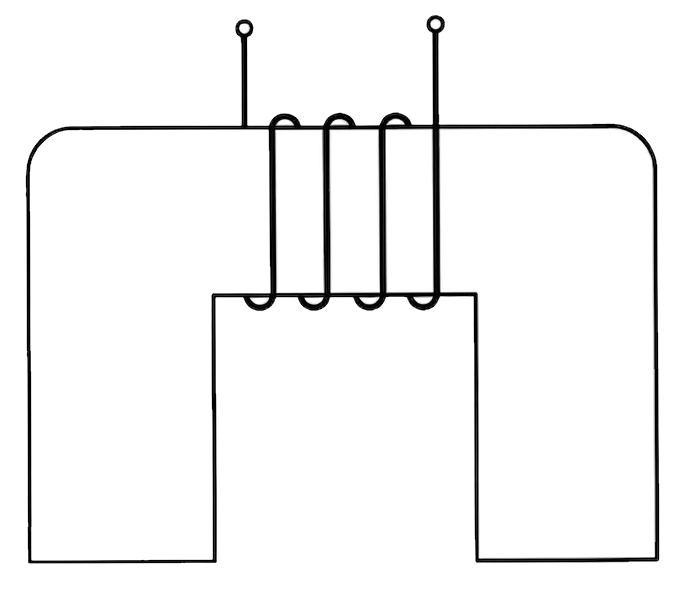
\includegraphics[scale=0.3]{electroaimant_u_inverse_1.png}
%	\caption{Mon image}
\end{figure}
\vspace{1.5cm}
\begin{parts}
	\part[1] Imposer la polarité positive de la source de tension sur la borne de gauche.
	\part[1] Inscrire les pôles magnétiques (N et S) aux extrémités de l'électroaimant.
	\part[1] Tracer les lignes de champ magnétique à l'intérieur et à l'extérieur, en précisant leur sens de circulation.
	\part[3] Détailler le mécanisme physique d'aimantation par influence qui permet l'attraction d'un corps ferromagnétique par l'électroaimant.
	\part[3] Déterminer les pôles magnétiques résultants apparaissant sur un induit ferromagnétique placé face à l'aimant.
	\part[3] Citer deux méthodes permettant de démagnétiser un aimant permanent.
	\part[3] Est-il possible d'isoler le pôle d'un aimant (existence de monopôles) ? Justifier.
	\part[3] Quelle est l'influence d'un matériau amagnétique (comme l'aluminium) sur un champ magnétique ?
	\part[3] Citer trois propriétés fondamentales des lignes de champ magnétique.
	\part[3] Définir le flux magnétique $\Phi$, son symbole et son unité légale.
	\part[3] Définir l'induction magnétique $B$, son symbole et son unité légale.
	\part[3] Expliquer à quoi correspond le phénomène de saturation magnétique d'un matériau.
	\part[3] Donner la relation mathématique entre l'induction $B$, le flux $\Phi$ et la section $S$.
	\part[3] Citer une application utile des courants de Foucault et un cas où ils sont indésirables.
	\part[3] Expliquer l'effet de l'insertion d'un noyau de fer dans une bobine sur la valeur de l'induction $B$.
\end{parts}
\vspace{0.5em}
\needspace{50\baselineskip}
\begin{solution}
	\begin{center}


%\begin{figure}[ht]
	\centering
	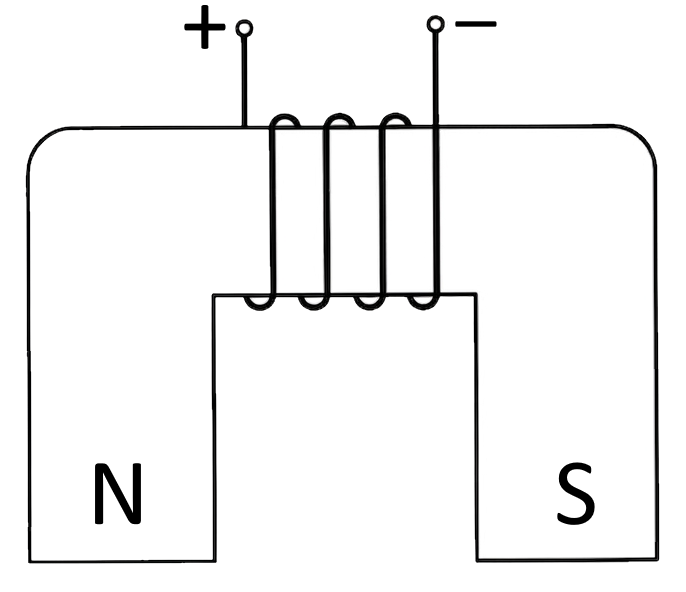
\includegraphics[scale=0.3]{electroaimant_u_inverse_N_S_reponse.png}
%\end{figure}
	\end{center}

\begin{align*}
	&\text{a) La borne (+) est reliée au côté gauche de l'enroulement.} \\[6pt]
	&\text{b) Par la règle de la main droite, le pôle Nord (N) est identifié là où le flux sort.} \\[6pt]
	&\text{c) Les lignes vont du Nord vers le Sud à l'extérieur du noyau et du Sud vers le Nord à l'intérieur du noyau.} \\[6pt]
	&\text{d) L'induction de l'aimant oriente les domaines magnétiques du matériau ferromagnétique, } \\
	&\text{créant des pôles opposés face à face qui génèrent la force d'attraction.} \\[6pt]
	&\text{e) Un pôle Sud apparaît face au Nord de l'aimant, et un pôle Nord face au Sud.} \\[6pt]
	&\text{f) Méthodes de démagnétisation : élévation de température (point de Curie) ou chocs mécaniques.} \\[6pt]
	&\text{g) Non, si un pôle Nord existe, un pôle Sud existe obligatoirement.} \\[6pt]
	&\text{h) Un matériau amagnétique n'a aucune influence sur le champ magnétique.} \\[6pt]
	&\text{i) Propriétés : boucles fermées, ne se croisent jamais, sortent perpendiculairement aux pôles.} \\[6pt]
	&\text{j) Le flux } \Phi \text{ représente l'ensemble des lignes de champ. Unité : Weber \qty{}{[\weber]}.} \\[6pt]
	&\text{k) L'induction } B \text{ est le nombre de lignes par unité de surface. Unité : Tesla \qty{}{[T]}} \\[6pt]
	&\text{l) La saturation est l'état où une augmentation de l'excitation } H \text{ n'augmente plus } B  \\[6pt]
	&\text{m) Relation fondamentale : } B = \dfrac{\Phi}{S} \unit{[\tesla]} \\[6pt]
	&\text{n) Utile : freinage (ralentisseurs). Indésirable : pertes dans les transformateurs.} \\[6pt]
	&\text{o) Le noyau de fer renforce considérablement l'induction } B \text{ par rapport à l'air.}
\end{align*}
\end{solution}	
\end{questions}
\end{document}